\begin{figure}[h]
    \begin{subfigure}[b]{\linewidth}
        \centering
        % trim={<left> <lower> <right> <upper>}
        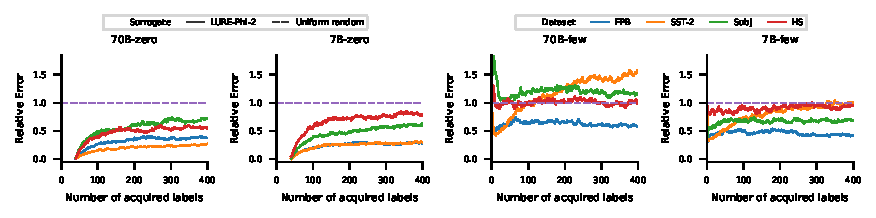
\includegraphics[width=\linewidth,trim={0 5pt 0 0}]{
            figures/pdf/relative_errors_phi2.pdf
        }
        \caption{Llama 2 target models and Phi-2 surrogate model}
         \label{fig:7b_70b_phi_unif_lure}
    \end{subfigure}
    \begin{subfigure}[b]{\linewidth}
        \centering
        % trim={<left> <lower> <right> <upper>}
        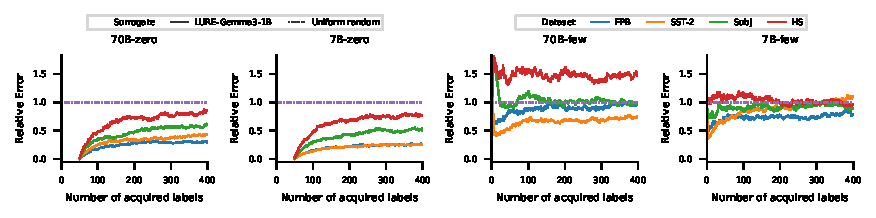
\includegraphics[width=\linewidth,trim={5pt 5pt 0 0}]{
            figures/pdf/relative_errors_gemma_1b.pdf
        }
        \caption{Llama 2 target models and Gemma3-1B surrogate model}
        \label{fig:7b_70b_gemma3_1b_unif_lure}
    \end{subfigure}
    \caption{
        Even very small surrogate models can support effective active testing in simple cases, although they struggle with evaluating our best-performing target model, 70B-few.
    }
    \label{fig:7b_70b_phi_gemma1b}
\end{figure}